\chapter{Introduction}

\section{What about it?}

The idea behind of the develop ot this software isn't only to do a
good tool for educational centers, is also an excuse to research and
learn about a lot of technologies and patterns but above all it's
about how to do clean, simple and easily readable sotware.

This software has been thinked to help a lot of teachers in their
work, but which is exactly the problem? And how it will help?

Until a few years ago the digitalization of education was something
imposible to think, the cost of equipments and the digital illiteracy
did imposible to think in to do things of another way. The only computers
that we could see was inside the 'Computer room', where students learnd
to use a simple text processor, received a simple notions of internet
of websites, mail system or storage devices, isn't bad to start, but
we don't talk about this. And what about teachers? Maybe a few of
computers in some rooms or office allow them send mails, maybe build
a simple website or offers some resource to the students (in the better
case). As we can imagine, the paper was the mainly support of all
about management of the center.

If we think about proccesses in a scholar center we can't imagine
the amount of paper that is necesary to registry all about students,
teachers, subjects, relationships between them and the rest of work.
And the worst of this is that every three months and every year the
most of this documents, papers, records, etc, need be redo, because
the mayority of this relations will change and will be necesary record
all.

Can you imagine the amout of papers, time and efforce is necesary
to do this? We will talk more about this after.

So now all peple have a smarphone, the hardware is really cheap (laptops,
tablets, etc...) and open a website for a inexperted person is very
easy, and almos free, in some clicks. There are alot of system and
tools about e-learning like Moodle, Chamilio , etc that allows manage
a lot of thigs like classroom, activities, exams, ect... all had been
listen somethimes about it but they have an specific domain and are
builded to an specific way.

This area is more or less knowled for the mayority of new teachers
and schooll stuff. Many center uses some tools like this to do a lot
of tasks, but in spite of it, there are another a lo of tool much
very heavy that is following hand made.arises

\section{Why to build a new tool?}

But is really necesary build to zero a new tool for do this. Well,
if we want, could reuse some preexisintg tool, maybe adding some module
to do all things that we detect that fault, but this present a lot
of problem, that are closely related with the architecture and liceses
of this software. Because of this, is putted a lot of effor in this
project in the opennes of code and architecture, beause this is that
make possible that the platform can be change, evolutionate in many
forks and feedback herself.

\section{Domain of the problem}

The idea to build SMS arises from the need of a managment system for
a specific educational center in Granada, that mainly speed up all
their internall management, avoid the spend of printed paper and save
huge amounts of time. Beside this they want a system that was helpful
for making better management decisions, in marking paths for future
improvements.\bigskip To achieve that the system would need as core
a subsystem of relationships managment, teachers that imparts class
to students, students that are enrollments in subjects and in groups
or courses, and a long etcetera. This only as the base of the system,
because with this would only be modeled the kind of relations that
the center have. A part of this and like the minimal requirements
the center need that the sistem provide a simple way to do their most
heavy and paper, time and money cost, the attendance contros (we can
start to see some requirements that the system would have). Appart
of this but related they need a system to save marks related with
students and disciplinary notes. Only this three things done digitally
may be a small internal revolution.

\section{The cost of non-digitalization}

Many times we do not perceive the cost of the processes in which we are involved
because we do not pay directly this cost or because we are so used to it that is
not evident.

\subsection{Paper}

How many papers are spended by a normal teacher in a high?


\subsubsection{Standard controls}

Marks and nottations.

If we think that a normal teacher have a 8 groups of students (if it works in a
full time) ,  this means 25 houres approximately at week, and each group have
25-30 student of average. In all there are 200 students which a teacher have relation.

Each educational center have a own control sytem but normally and like is in this
case, there are a lot of standard document that each teacher manages to follow
the evolution of their students.

We are going to make the calculus of  these through the summary of the mainly
processes that they do.

To begin each teacher need to follow the evolution of each children in their
subject quarterly, to do this they uses an official document where they write
all interesting anotations about the student, from marks of partials or final
exams to marks about homeworks or class issues.

If the common teacher (here "teacher") have 200 students make up a total of 600
pages. Normally each center give to teacher a book with all this pages officialley
formated to this task.





\subsubsection{Tutorizing}

Each time that a parent want to check the evolution of his son  . Mas

30 estudiantes por 3 reuniones con padres, por 14 papeles por
asignatura es igual a : 1260 pages.



Tutorias, dos hojas de info peronsal, hoja de tutoria por asignatura , 10 subject
per boy, ms otras dos hojas para la pedagoga.



\subsubsection{Delays}

Retrasos, con otro papelito.

5 per week, per 32 weeks: 160 pages


\subsubsection{Class attendances}

All weeks all teachers that impart class to a group write in a paper
all attendance controls of a class (independly of theri own records). This
is does between all teachers. So, in on avergae a center have around 1000 students
and around 25 students by course, more or less 40 courses and is neccesary
an attendance records paper by class, so is equal to 40 documents per week and
if the course have 32 weeks, the result is aproximately 1280 sheets of paper.



\textbf{Another center communications}
Nofifications
Reports
Evaluations


\textbf{Summarize}

With the follow constraint:

\begin{itemize}
\item A scholar course have 32 weeks at year on average (32-36 with 160-180 days).
\item The cost by printed page is about 0.03 cents of euros.
\end{itemize}


So, with this we can obtains this conclusion.

\begin{table}[H]
\centering

\begin{tabular}{@{}lllllll@{}}

Process & Per week  & Per year  & Cost  \\
\midrule

Class attendance  &  40  &  1280  &   38,4   \euro  \\

%Admin       &  3   &  10    &   270 h   & 15 \euro  & 4050   \euro  \\
%Direction   &  4   &  10    &   360 h   & 20 \euro  & 7200   \euro  \\

\midrule
& & & & Total & 38250 \euro \\
\end{tabular}
\caption{Equivalent stuff cost in managment tasks. }
\label{my-label}
\end{table}




\subsection{Time and Money}

Is not only the cost of the material resources, is also the time and their money
equivalence what we are trying to save.  If we count the hours of work that a
common teacher dedicate to do this we can estimate the cost that all student
managment related work required.

\begin{table}[H]
\centering

\begin{tabular}{@{}lllllll@{}}

Stuff & Amount & Hours/Month & At year & Price Hour & Total  \\
\midrule

Teacher     & 40 & 5    & 1800 h   & 15 \euro  & 27000  \euro  \\
Admin       & 3  & 10   & 270 h   & 15 \euro  & 4050   \euro  \\
Direction   & 4  & 10   & 360 h   & 20 \euro  & 7200   \euro  \\

\midrule
& & & & Total & 38250 \euro \\
\end{tabular}
\caption{Equivalent stuff cost in managment tasks. }
\label{my-label}
\end{table}

This would be the cost if we think in the hours that all school stuff spend
in this kind of tasks and that are not been spended in projects of the own
center.
Can you imagine the amount of projects that would be doing with this huge
amount of houres of work by the stuff of the center?

The problem is allways the same, organization, control, and focused value. And
the common patter is not have a control over all and as thinks as this, the
companies lost alot of money and resources. The control of that happens in your
bussines is the most important and obviously is the only way to can take
decissions data based.

\subsection{Value of business}
Another thing that does go unnoticed is about the values of the data that a big
relational centers as school manage without any insight of their value.
In a standar center with 1000 students is generated around 10.000 records per
month, with a records schemas very basic. It is around 90.000 records per year
and if we have a more complex system with a lot data recorded the amount can be upper.
So, what happens with all of this data. There are any value? Obviously yes,
the explotation of this data is not very clear at first because the most of
people (centers directives included) not seen the center as a business, which
actually it is, only that our product is the quality of the teaching that we are
offering to our students.
So, as in any manufactured process there are a lot of steps that can be improved,
only if are controlled and measured. With students is the same (without any wrong
charm), there are a lot of steps, processes and stages that could be improved to
offer a better education.
If we detect that by whatever reason a student have a bad trend in their evolution
is very difficult to detect if we don't have a strong system to recollect data
and be able to do a fast actuation (proactive in oposite of late traditional
reactive behaviour) will be very difficult fix the problem.
And as there are a huge amount of data is difficult that anyone can process this
manually, and by this reason, is not easy too detect what part of our processes
fail or need to be improved.
All this problem can be easily solved with a powerfull system that can be recollect,
processes and give human-readable way all the conclusion obtained.
And this the other big mission of the kind of software like this, offer a
bunisses value of the data that help to manage.

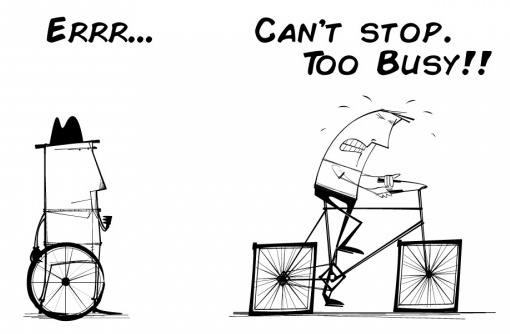
\includegraphics[scale=0.5]{img/toobusytoimprove.jpeg}


\section{State of Art }

As part of the research process has been analyses some aplications
that (although isn't a directly competition) represent the actual
state of art about the kind of sofware we are talking about.


\begin{table}[]
\centering

\begin{tabular}{@{}lllllll@{}}

Feature & classDojo & TeacherKit & A+ & iDoceo & Additio & SMS \\ \midrule

Attendance & \completeValue & \completeValue & \completeValue & \completeValue & \completeValue & \completeValue \\

Discipline & \partialValue & \completeValue & \completeValue & \completeValue & \completeValue & \completeValue \\

Attitude & \partialValue & \completeValue & \completeValue & \completeValue & \completeValue & \completeValue \\

Marks & \noneValue & \completeValue & \completeValue & \completeValue & \completeValue & \completeValue \\

Competencias & \noneValue & \noneValue & \noneValue & \completeValue & \completeValue & \completeValue \\

Rubrics & \noneValue & \noneValue & \noneValue & \completeValue & \completeValue & \completeValue \\

Message & \completeValue & \completeValue & \completeValue & \noneValue & \noneValue &	\completeValue \\

patters & \noneValue & \noneValue & \noneValue & \completeValue & \completeValue & \completeValue \\

reports & \noneValue & \completeValue & \completeValue & \partialValue & \completeValue & \completeValue \\

analysis & \partialValue & \completeValue & \partialValue & \partialValue & \partialValue & \completeValue \\

models and predictions & \noneValue & \noneValue & \noneValue & \noneValue & \noneValue & \completeValue \\

Centralizate and jerarqy & \noneValue & \partialValue & \noneValue & \noneValue & \noneValue & \completeValue \\ \midrule

Total & 58.3\% & 80.5\% & 72.2\% & 	72.2\% & 80.5\% & 99\% \\
\end{tabular}
\caption{Features}
\label{my-label}
\end{table}


\begin{table}[]
\centering

\begin{tabular}{@{}lllllll@{}}

Feature & classDojo & TeacherKit & A+ & iDoceo & Additio & SMS \\ \midrule

Personalization & \noneValue & \noneValue & \noneValue & \noneValue & \noneValue & \noneValue \\

Good UI & \partialValue & \completeValue & \completeValue & \completeValue & \completeValue & \completeValue \\

Buena UX & \partialValue & \completeValue & \completeValue & \completeValue & \completeValue & \completeValue \\

Price & \noneValue & \completeValue & \completeValue & \completeValue & \completeValue & \completeValue \\

Performance & \noneValue & \noneValue & \noneValue	 & \completeValue & \completeValue & \textcolor{ownGreen}{\completeValue} \\

Scalable & \noneValue & \noneValue & \noneValue & \completeValue & \completeValue & \completeValue \\

Data control & \completeValue & \completeValue & \completeValue & \noneValue & \partialValue & \completeValue \\

Multiplatform & \noneValue & \noneValue & \noneValue & \completeValue & \completeValue & \completeValue \\

Centralized & \noneValue & \completeValue & \completeValue & \partialValue & \completeValue & \completeValue \\ \midrule

Total & 44.4\% & 50.0\% & 16.6\% & 	16.6\% & 44.4\% & 99\% \\
\end{tabular}
\caption{Architecture and design}
\label{my-label}
\end{table}

Let's go to start!
